% ================================================================
%  conteudo/resultados.tex
% ================================================================

\section{Resultados e Discussão}

\subsection{Determinação da Biomassa Seca}

Após o cultivo de \textit{Saccharomyces cerevisiae} ATCC~7754 em meio YM por 27 horas a 30~°C e 100~rpm, determinou-se a concentração de biomassa seca a partir de triplicatas de 10~mL de suspensão celular. A Tabela~1 apresenta as massas e concentrações obtidas para cada tubo.

\begin{table}[H]
\caption{Determinação da biomassa seca de \textit{S. cerevisiae} por método gravimétrico}
\centering
\begin{tabular}{cccccc}
\toprule
\textbf{Tubo} &
\textbf{Massa tubo (g)} &
\textbf{Massa total (g)} &
\textbf{Biomassa (g)} &
\textbf{Volume (L)} &
\textbf{Concentração (g/L)} \\
\midrule
1 & 5,5054 & 5,5341 & 0,0288 & 0,010 & 2,88 \\
2 & 5,3165 & 5,3420 & 0,0273 & 0,010 & 2,73 \\
3 & 5,4825 & 5,5095 & 0,0270 & 0,010 & 2,70 \\
\midrule
\multicolumn{5}{r}{\textbf{Média}} & \textbf{2,77} \\
\bottomrule
\end{tabular}
\end{table}

A média das três determinações foi de 2,77~g/L, valor adotado como concentração da solução principal para o cálculo das diluições subsequentes. A boa reprodutibilidade entre os tubos, com variação inferior a 0,2~g/L entre os extremos, indica que o procedimento gravimétrico foi conduzido com adequado controle experimental.

\begin{figure}[H]
\centering
\caption{Biomassa de \textit{Saccharomyces cerevisiae} ATCC~7754 obtida após centrifugação e secagem}
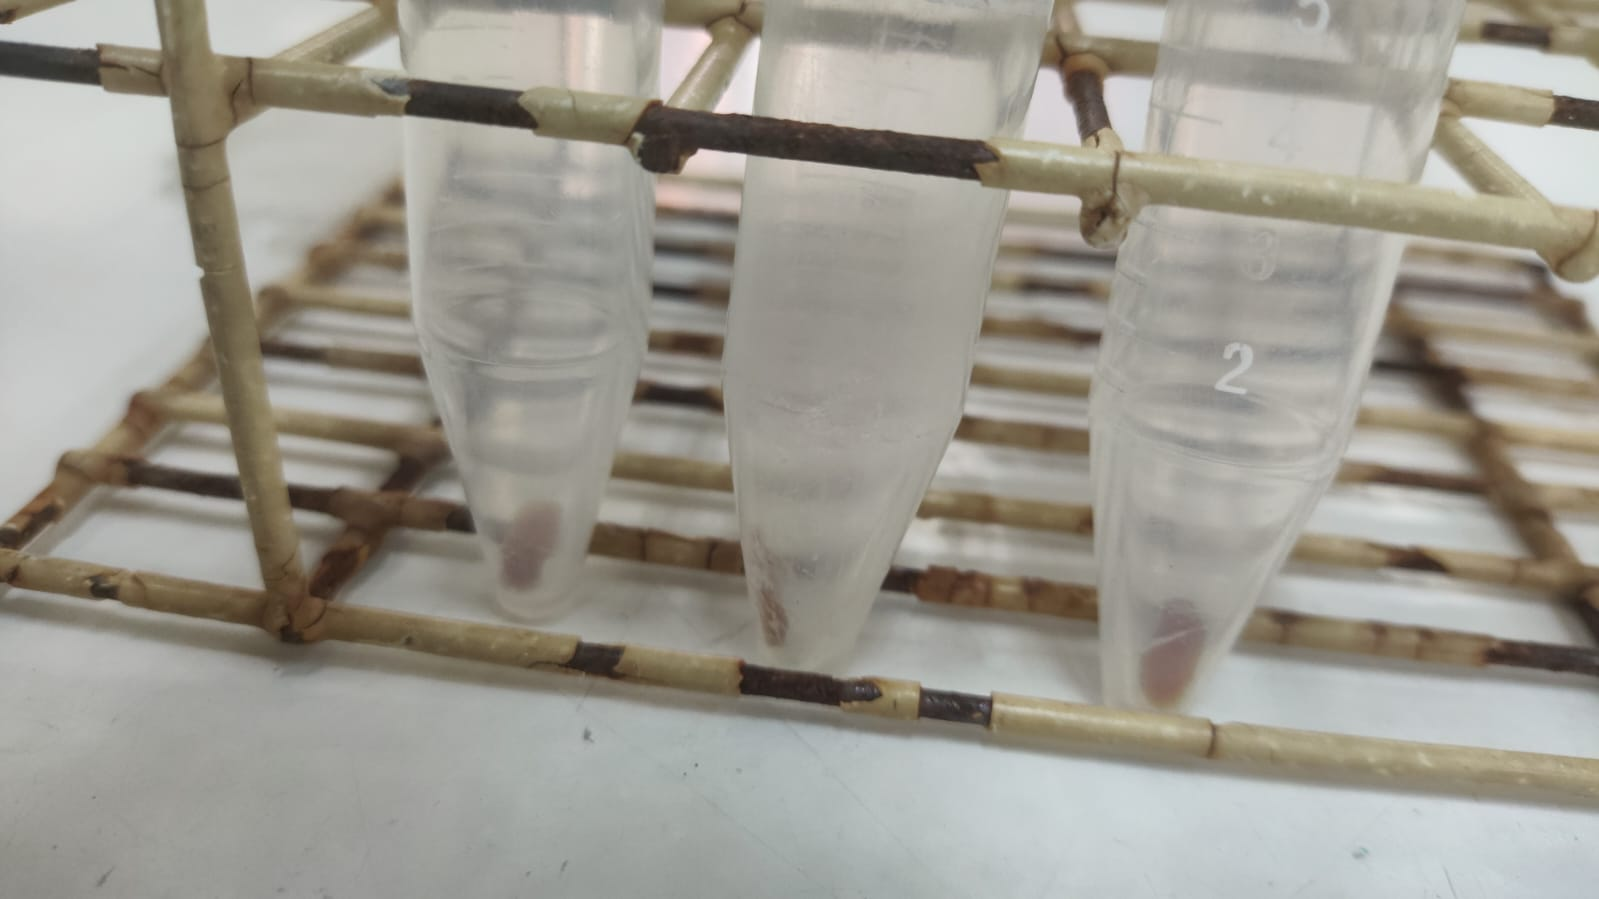
\includegraphics[width=0.5\textwidth]{image/biomass.jpeg}
\end{figure}

\subsection{Medidas de Absorbância por Turbidimetria}

A partir da solução principal, foram preparadas diluições com fatores de 5, 10, 15, 25, 50 e 100. Para cada diluição, mediu-se a transmitância (\%T) tanto da suspensão celular quanto do sobrenadante, e calcularam-se as respectivas absorbâncias. A absorbância corrigida foi obtida pela diferença entre a absorbância da suspensão e a do sobrenadante, eliminando a contribuição dos componentes do meio YM na leitura. A Tabela~2 consolida os resultados obtidos.

\begin{table}[H]
\caption{Transmitâncias e absorbâncias medidas por fator de diluição}
\centering
\begin{tabular}{cccccc}
\toprule
\textbf{FD} &
\textbf{\%T suspensão} &
\textbf{Abs. suspensão} &
\textbf{\%T sobrenadante} &
\textbf{Abs. sobrenadante} &
\textbf{Abs. corrigida} \\
\midrule
5   & 18,12 & 0,7418 & 97,95 & $8,99 \times 10^{-3}$ & 0,7328 \\
10  & 59,55 & 0,2251 & 98,85 & $5,03 \times 10^{-3}$ & 0,2201 \\
15  & 39,70 & 0,4012 & 99,40 & $2,61 \times 10^{-3}$ & 0,3986 \\
25  & 65,57 & 0,1833 & 99,20 & $3,48 \times 10^{-3}$ & 0,1798 \\
50  & 81,95 & 0,0865 & 99,85 & $6,51 \times 10^{-4}$ & 0,0858 \\
100 & 91,25 & 0,0398 & 99,95 & $2,17 \times 10^{-4}$ & 0,0396 \\
\bottomrule
\end{tabular}
\end{table}

O sobrenadante apresentou absorbância mensurável em todas as diluições, porém com valores substancialmente inferiores aos da suspensão celular, o que confirma que a turbidez observada é atribuída predominantemente à presença de células. Nas diluições mais elevadas (FD=50 e FD=100), a contribuição do sobrenadante torna-se proporcionalmente mais relevante, reforçando a importância da leitura corrigida para garantir a acurácia da curva padrão (MIRA et al., 2022).

\subsection{Curva Padrão e Ajuste Linear}

A correlação entre os valores de absorbância corrigida e as concentrações de biomassa revelou comportamento linear ao longo de toda a faixa avaliada, conforme evidenciado pela Figura~2. O ajuste linear aos dados experimentais resultou na equação apresentada na Equação~\ref{eq:curva_padrao}, com coeficiente de determinação R²~=~0,9935, indicando que 99,35\% da variação nos dados é explicada pelo modelo linear proposto.

\begin{equation}
    C = 0{,}7501 \cdot A_{600} - 0{,}0079
    \label{eq:curva_padrao}
\end{equation}

em que $C$ é a concentração de biomassa em g/L e $A_{600}$ é a absorbância corrigida medida a 600~nm.

\begin{figure}[H]
\centering
\caption{Curva padrão para quantificação de biomassa de \textit{Saccharomyces cerevisiae} ATCC~7754}
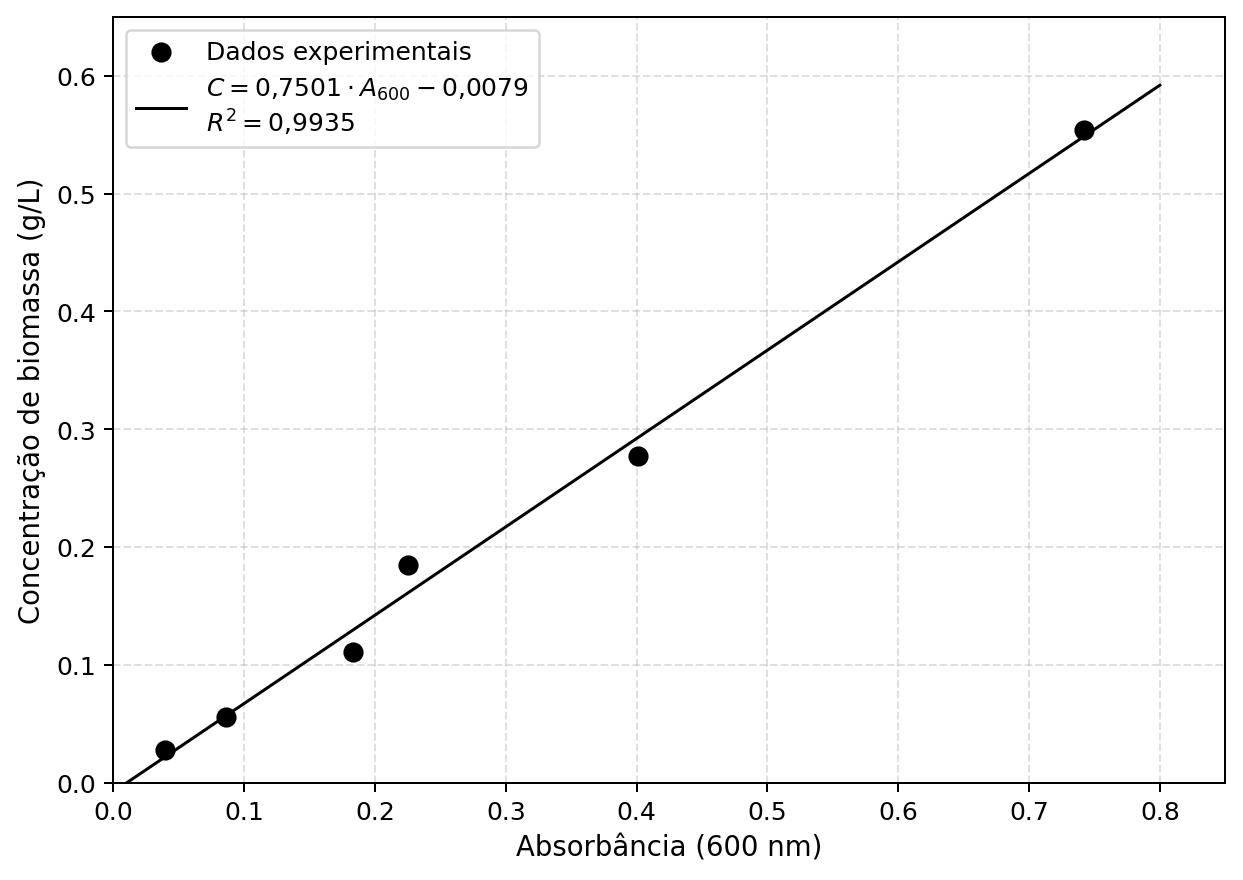
\includegraphics[width=0.75\textwidth]{image/curva_padrao.png}
\end{figure}

O elevado valor de R² confirma a validade da correlação linear entre a densidade óptica e a concentração de biomassa seca na faixa avaliada, em conformidade com os limites de linearidade da Lei de Beer-Lambert para suspensões celulares homogêneas (MIRA et al., 2022). A proximidade do intercepto com zero ($-$0,0079~g/L) reforça a consistência física do modelo, uma vez que a ausência de células deveria corresponder a absorbância nula.
